\documentclass[11pt,a4paper]{ivoa}
\input tthdefs

\usepackage{array}
\newcolumntype{L}{>{\centering\arraybackslash}m{3cm}}

\title{Vodml-instance-vot}

% see ivoatexDoc for what group names to use here
\ivoagroup{DM}


\definecolor{gray}{rgb}{0.4,0.4,0.4}
\definecolor{darkblue}{rgb}{0.0,0.0,0.6}
\definecolor{maroon}{rgb}{0.5,0,0}
\definecolor{cyan}{rgb}{0.0,0.6,0.6}

\lstset{
  basicstyle=\ttfamily,
  columns=fullflexible,
  showstringspaces=false,
  commentstyle=\color{gray}\upshape
}

\lstdefinelanguage{XML}
{
  morestring=[b]",
  morestring=[s]{>}{<},
  morecomment=[s]{<?}{?>}, 
  morecomment=[s]{<!--}{-->},
  stringstyle=\color{black},
  identifierstyle=\color{darkblue},
  keywordstyle=\color{maroon},
  morekeywords={ref,utype,dmrole, dmtype, value}% list your attributes here
}
\author{François Bonnarel}
\author{Gilles Landais}
\author{Laurent Michel}
\author{Jesus Salgado}

\editor{Laurent Michel}

% \previousversion[????URL????]{????Concise Document Label????}
\previousversion{This is the first public release}
       

\begin{document}
\begin{abstract}
???? Abstract ????
\end{abstract}


\section*{Acknowledgments}

???? Or remove the section header ????

\section*{Conformance-related definitions}

The words ``MUST'', ``SHALL'', ``SHOULD'', ``MAY'', ``RECOMMENDED'', and
``OPTIONAL'' (in upper or lower case) used in this document are to be
interpreted as described in IETF standard RFC2119 \citep{std:RFC2119}.

The \emph{Virtual Observatory (VO)} is a
general term for a collection of federated resources that can be used
to conduct astronomical research, education, and outreach.
The \href{http://www.ivoa.net}{International
Virtual Observatory Alliance (IVOA)} is a global
collaboration of separately funded projects to develop standards and
infrastructure that enable VO applications.


\section{Introduction}
The first purpose of a model is to provide,  for a particular domain, a formal description of the relevant quantities and of the way they are linked together .
This documentary role facilitates the communication between the stackholders and thus the design of interoperability protocols. 

At data level, the interoperability consists in arranging searched data in a way that a client can understand them without taking care of their origin. So that, the same code can process and compare data coming from different sources.  That way to arrange data is given by the model.

This is not easy to do with VOtables because VOTables are containers. The VOTable schema cannot say how data are mapped onto a model or whether they match any model either. This is not a problem for simple protocol responses (ref) because the VOTable structure is defined by the protocol itself but this is however a big issue for VOTables containing native data such as Vizier queries or TAP response.

The challenge here is to bind native data with a given model in way that a model aware software can see them as model instances while maintaining the possibility to access them in their original forms.
This is partially done with UTypes that connect FIELDs or PARAMs with model leaves. Unfortunately, there is no standard way to construct UTypes and thus to parse them. This is just because UTypes have been invented at a period when there was no standard way to serialize model.

The VODML (ref) standard, REC since 2016,  is a meta-model that gives a standard way to design VO models and to make them machine-readable. In VODML, model leaves are no longer identified by long strings denoting the path through the model (Utypes) but by their location in the model hierarchy.
The consequence is that an annotation mechanism based on VODML must be able to reconstruct the model hierarchy. This is very interesting because a copy the model hierarchy with leaves set with real data is nothing else that a model instance which is exactly what we need to be interoperable.

The idea of the VODML mapping is to insert on the top of the VOTable an XML block denoting the model structure and containing references to the actual data.
So that, to build an model instance, the model-aware client has just to make a copy of that structure and to resolve the references. Other clients can just ignore the mapping block. This approach, has been proposed by (GL and OL). 

We have tested the syntax originally proposed and it turned out that it was not well suited for archival data or for TAP responses where the annotation process must be automated as much as possible (entirely for TAP). 

Vodml-instance-vot is based on the same principles as the original proposal but with a particular concern for the annotation of archival data by keeping focused on both client needs and easiness of the annotation process.
This requires the syntax to be as simple as possible and as flexible as possible to be usable with a wide range of data sets.
Vodml-instance-vot  has been built upon 3 basic elements (simple values,  tuples and  lists, like JSON)  plus a few others annotations guiding the parser.
The connections with the data are setup by XML element attributes, so that the mapping tree just depends on the model but not on the mapped data.

These ideas were first tested in the framework of the TDIG on VOTABLEs containing time series provided by different missions such as Gaia or ZWICKI. Then the syntax has been refined to be used to validate the Mango model on real data.

\iffalse
 The annotation process 

we though it was woth, has been tested on various data. We reached the conclusion that the annotations was not well suited for archival data.

 

 UTypes have been replaced with short identifiers which role depends on 


This is legacy from a period 
This is why the Utype based data annotation has been withdrawn

This is partially done with GROUPs that allow to gather FIELDs and PARAMs into hierarchical structures. Unfortunately, the model elements, in the current VOTable spec (ref) are identfied by Utypes. There is no standard way to construct UTypes and this to parse them. In other, client software has to manage UType list. IN fact 

If  


This can be achieved at protolol level by having a 1-1 association between protocol and  model. With this approach, used for all VO simple protocols (ref), the query responses have a fixed format to which the data must conform. The VOTable FIELDs and PARAMs are defined by the protocol.


associating one model with
The model can also be used by the data provider to expose data in a view
This scope can be extended if we make the model machine readable.


There is no VO standard specifying how to map real data on a model. 
This shortcoming is a bottleneck for interoperability since there is no clean way to compare the same quantities but from differents datasets. 


The model mapping currently used is based on GROUPs. GROUP is a VOTable feature that allows to gather FIELDs and PARAMs into hierarchical structures. In theory, this could be used to map models. Unfortunately, in VOTables, GROUPS haven been used long time before we a standard  

This is satisfactory in many cases but with some limitations however:\begin{enumerate}
   \item The GROUPs, as they are currently used, do not reflect the complete model structure. The are mostly used to group columns with a loose coupling with the model hierarchy. This prevents the restore complex data structures.
   \item The identification of the GROUP elements is based on Utypes which are not clearly connected with the underlying model. Utypes are actually used to represent simple structures. In the current implementations, the client knows the data structures (e.g. coordinate system) and pick values within the group to fill them..
\end{enumerate}
These limitations were unavoidable while we had no common way to represent  models. It is indeed difficult to imagine a consistant model mapping mechanism if there is no standard serialization schema for those models. The situation changed with the usage of VODML. VODML proposes a robust way to make models machine-readable. With VODML, we can consider a mapping syntax directly derived from the model serialization. There are 2 approaches that might be complementary. 
\begin{enumerate}
   \item The first option is to hide the model complexity by flattenning its representation. This is the way GROUPs do work. This approach has the advantage of being compact but it has some strong limitations such as the impossibility of having different elements playing the same role (e.g. 2 position columns in the same table)
   \item The second option consists in keeping the model structure even if this leads to more complex annotations.
\end{enumerate}


Vodml-instance-vot is based on the second option with a particular concern for the process of archival data annotation. The purpose of the VODML mapping in VOTables is to provide a bridge between the data and the model it refers to. The goal of the mapping processing is to make possible to build instances set with values taken out the data tables. In theory, a perfecly faith mapping should be capable of rendering any model feature. In our opinion this ambitious goal led to a mapping syntax difficult to manage.
We prefer to discard this round-trip requirement and to keep focused on both client needs and easiness of the annotation process.

Our main use case is the annotation  of pre-existing data. This  means the annotation process must succeed whatever the way data are arranged even if they do not contain all quantities requested by the model.  
We consider that we have to provide clients with both a data hierarchy view as simple as possibel and an accurate description of the used coordinate systems. 

For most of the usages (display, plot, match, computation),  complex data hierarchies can be wrapped in 3 basic types, the simple values,  tuples and  lists. Vodml-instance-vot  has been built upon these 3 types with a few others annotations guiding the parser.

These ideas that led to this proposal were first tested in the framework of the TDIG on VOTABLEs containing time series provided by different missions such as Gaia or ZWICKI. Then the syntax has been refined to be used to validate the Mango model on real data.

\fi
%The identification of the GROUP elements is based on Utypes which are not clearly connected with the underlying model. Utypes are actually used to represent simple structures. In the current implementations, the client knows the data structures (e.g. coordinate system) and pick values within the group to fill them..



%The current proposal 



%This standard comes after many discussions in the VO about the syntax to be used to annotate VOTable. 
%The ideas that led to this proposal were first tested in the framework of the TDIG on VOTABLEs containing time series provided by different missions such as Gaia or ZWICKI. Then the syntax has been refined to be used to validate the Mango model on real data.

%The existing mapping based on GROUP works fine with the simplest cases. It has the disadvantage of being based on Utypes which are not clearly connected with the underlying model. Utypes are actually used to represent simple structures. In the current implementations, the client knows the data structures (e.g. coordinate system) and pick values within the group to fill them.

 %For now, mone discover or reconstruct a classe hierarchy from groups either. 
%The purpose of the VODML mapping in VOTables is to provide a bridge between the model it refers to and the data. The mapping processing is meant to deliver a model instance set with values taken out the data table. In theory, a perfecly faith mapping should be capable of rendering any model feature. In our opinion this ambitious goal led to a mapping syntax difficult to manage.
%We prefer to discard this round-trip requirement and to keep focused on the client needs and the easiness of the VOTable annotation process.

%ur main use case is the annotation  of pre-existing data. This  means the annotation process must succeed whatever the way data are arranged even if they do not contain all quantities requested by the model.  We consider that the client just needs to reconstruct the data hierarchy and to get a full description of the used coordinate systems. For most of the usages (display, plot, match, computation),  complex data hierarchies can be wrapped in 3 data types, the simple values, the tuples and the lists. The mango mapping has been built upon these 3 types with a few others annotations guiding the work of the parser.

\lstset{language=XML}

\subsection{Role within the VO Architecture}

\begin{figure}
\centering

% As of ivoatex 1.2, the architecture diagram is generated by ivoatex in
% SVG; copy ivoatex/archdiag-full.xml to archdiag.xml and throw out
% all lines not relevant to your standard.
% Notes don't generally need this.  If you don't copy archdiag.xml,
% you must remove archdiag.svg from FIGURES in the Makefile.

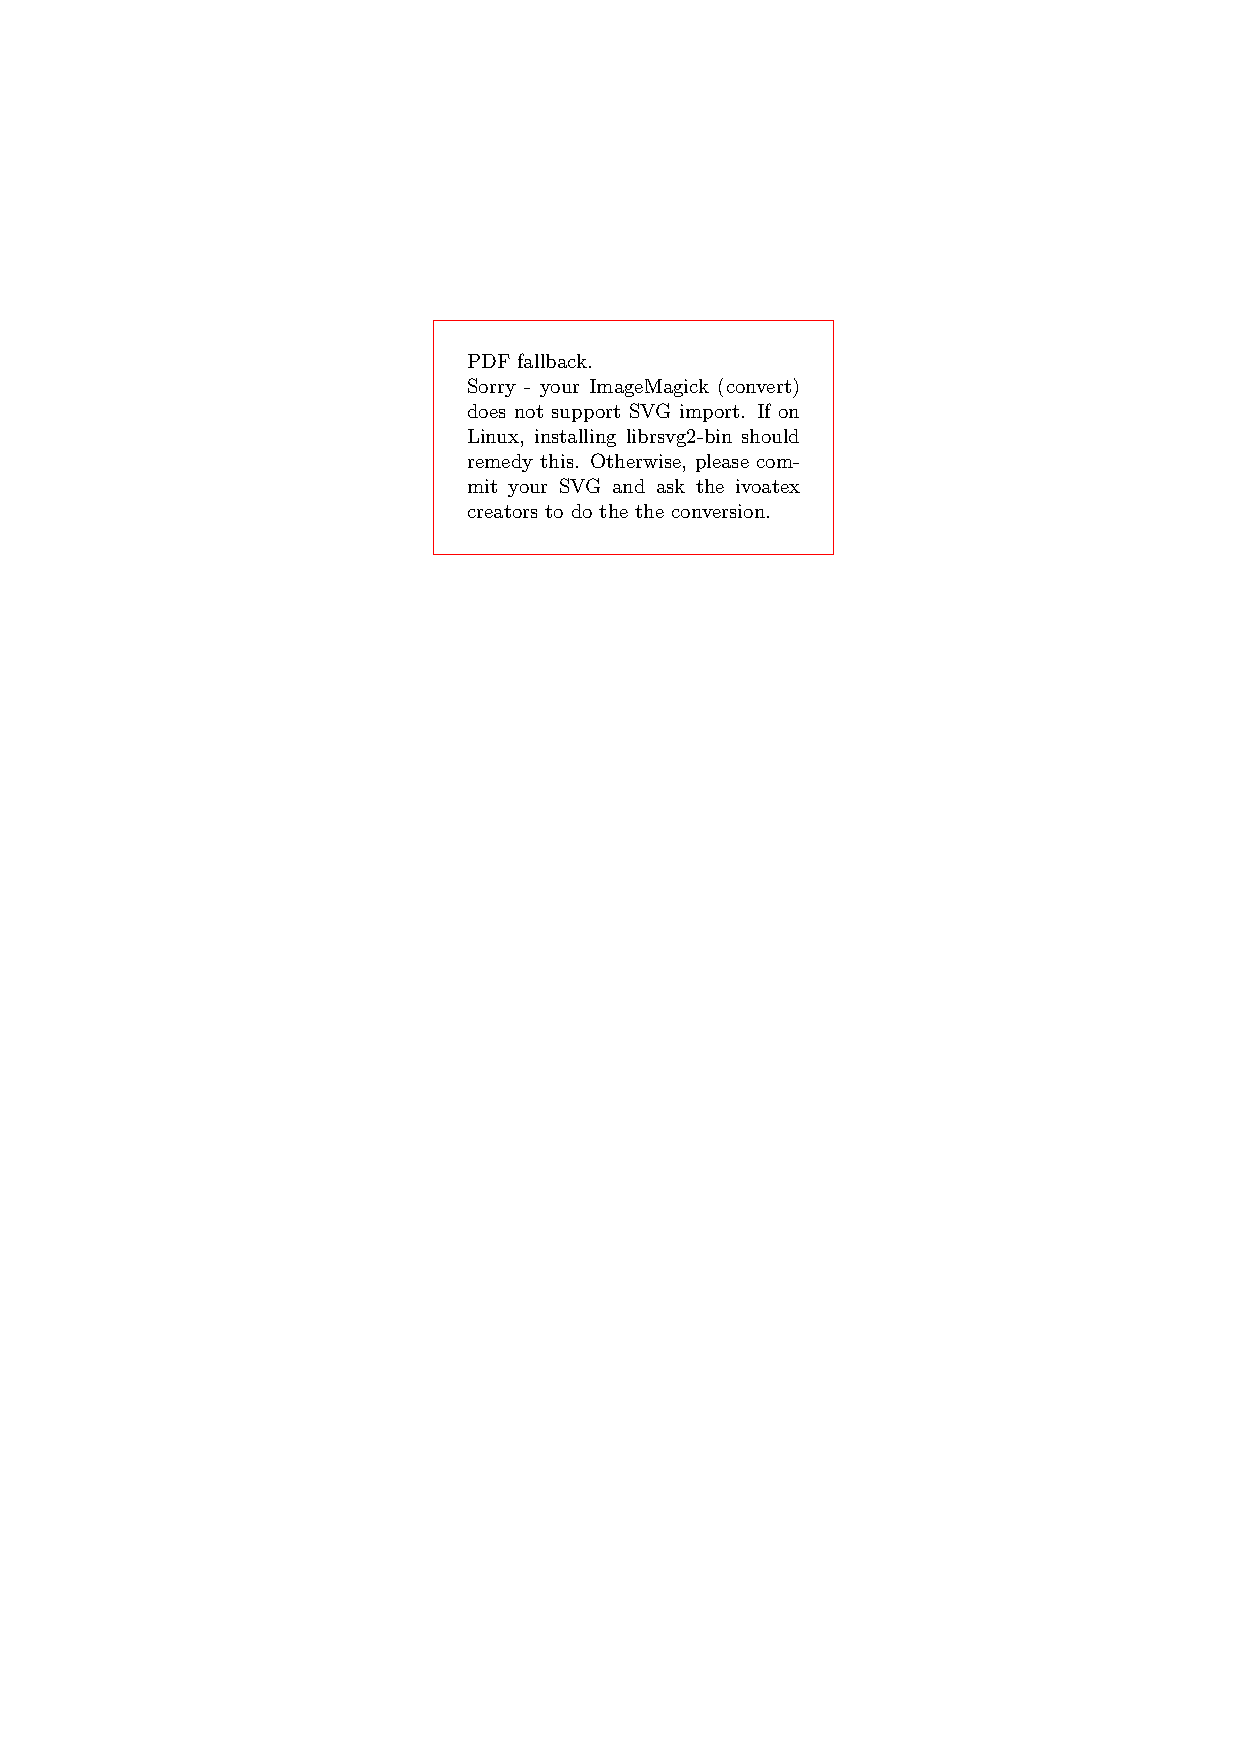
\includegraphics[width=0.9\textwidth]{role_diagram.pdf}
\caption{Architecture diagram for this document}
\label{fig:archdiag}
\end{figure}

Fig.~\ref{fig:archdiag} shows the role this document plays within the
IVOA architecture \citep{note:VOARCH}.

???? and so on, LaTeX as you know and love it. ????

\section{Use Cases and Requirement}

\subsection{Use Cases}

\subsubsection{Client Side}
The mapping is self consistant. The role of the mapping is to give the client all information it needs a reconstruct a datastructure similar to the model one. 
A model-aware client must be able to do this  this without implementing any code specific to any particular model.  The mapping syntax is independant of the model. The structure of the mapped model is given by the arrangement of the mapping elements, not by the elements them-self
.

\subsubsection{Server Side}
We have identified 3 sorts of servers that could annotate data:
\begin{enumerate}
   \item Mission data provider: the data annotation can be set once forever for each data product at the design phase.
   \item Archival data provider: The data annotation must be done for each archived datat set. The curator has a little control, on the data format and he/she has to do his best to math data with the model(s) 
   \item  TAP data provider: In case of TAP services, the annotation process in of charge of the TAP server that must match the queried data with the model quantities.
\end{enumerate}

The goal of the version is to support 1) and 2) with a special attention to facilitate 2). 3) is still an experimental feature at the time of this specification.

The annotation process can represent a significant extra work for the curator team that must be limited as much as possible. To do so the mapping syntax is designed to facilitate the use of templates. The structure of the mappinfg DOM does not depends on the way mapped data are arranged. The connection between  real data and mapping is done through XML elements attributes without changing the nature or the location of the mapping elements . 


\subsection{Requirements}

\begin{itemize}
\item Shy Annotations: The data mapping must not affect the operation of the existing clients

\item Faithful Annotations: The structure of the annotation must be faithful to any VODML compliant model. 


\item Different Usage Levels 
\begin{itemize}
   \item The data mapping must be easy to be ignored by the client
   \item The data mapping must allow clients to easily detect the model on which data are mapped
   \item The data mapping must allow clients to easily get the metadata (e.g. coordinate systems)
   \item The data mapping must allow clients to get full model instances for each table row
\end{itemize}

\item Easy to Build 
\begin{itemize}
   \item The mapping structure must be independant of the data structure
   \item The mapping syntax should facilitate the building of mapping components and templates.
\end{itemize}

\item Complex Data Mapping 
\begin{itemize}
   \item The mapping syntax must support to retrieve data over several tables
   \item The mapping syntax must be able to filter the data rows that are part of the current instance
   \item The mapping syntax must be able to group data rows in an set of instances
\end{itemize}
\end{itemize}

The syntax specified in this standard gives rules to build consistant annotations for any model. However, it do not prevent to do foolish things, the same way that a programming langage grammar does not prevent against irrelevant software.



%\begin{itemize}
%	\item This mapping syntax supports directive for the clients which are not part of the model (e.g. aggregation request or data filters).
%	\item The mapping as an explicit entry point, telling to the client what is the VOTable content.
%	\item Processing this alternate syntax require for the client to apply rules not states in the VOTable itself.
%\end{itemize}


\section{Syntax}

\subsection{Mapping Block Structure}

\textit{The rules below must be updated accordingly to the XML schema}

The mapping block is outside of the data tables. Its scope is the whole VOTable. Its stucture is given below.

\begin{lstlisting}[caption={INSTANCE bloc example},captionpos=b]
 <VODML>
    <MODELS>   ...  </MODELS>
    <GLOBALS>   ...  </GLOBALS>

    <TEMPLATES tableref=...>  ... </TEMPLATES tableref=...>
    <TEMPLATES tableref=...> ...  </TEMPLATES tableref=...>
    ...
 </VODML>
\end{lstlisting}

The mapping construction rules are the same whatever the model or the data layout are.

\begin{itemize}
    \item The mapping is located in a \texttt{<VODML>} block, child of \texttt{<VOTABLE>}.
    \item The mapping elements reflect the model structure.
    \item The \texttt{<VODML>} block starts with a list of implemented models.
    \item There is one \texttt{<TEMPLATES>} per mapped \texttt{<TABLE>}.
    \item There is one \texttt{<GLOBALS>} block containing data shared by the whole mapping.
\end{itemize}

\subsection{MODELS}

The models blocks contains the list of the models mapped in the block. Models referenced in \texttt{MODELS} are not necessary VO standards, but thet must be access through a VODML URI.

\subsection{GLOBALS}

Contains  \texttt{INSTANCE}s with that can be used everywhere in the \texttt{VODML}.


\begin{lstlisting}[caption={INSTANCE bloc example},captionpos=b]
  <GLOBALS>
    <INSTANCE ID="SpaceCoordFrame" dmrole="">
      <INSTANCE dmrole="coords:SpaceFrame.refPosition" dmtype="coords:StdRefLocation">
        <ATTRIBUTE dmrole="coords:StdRefLocation.position" dmtype="ivoa:string" value="NoSet"/>
      </INSTANCE>
      <ATTRIBUTE dmrole="coords:SpaceFrame.spaceRefFrame" dmtype="ivoa:string" value="ICRS"/>
      <ATTRIBUTE dmrole="coords:SpaceFrame.equinox" dmtype="coords:Epoch" value="NoSet"/>
    </INSTANCE>
    <INSTANCE >
      ... 
    </INSTANCE>
    ...
  </GLOBALS>
\end{lstlisting}

\texttt{INSTANCE}s contained in \texttt{GLOBALS} should have an  \texttt{@ID} attribute so that they can be referenced from other instances


\begin{table}[ht!]
     \begin{tabular}{|p{3cm}|p{7cm}|}
       \hline Child &  Role\\
       \hline  \texttt{INSTANCE}    &  Model instances with a scope covering the whole VOTable . \\       
       \hline 
     \end{tabular}
     \caption{Allowed  \texttt{GLOBALS} children} 
 \end{table}

 \texttt{GLOBALS} has no attributes. 


\subsection{TEMPLATES}

There is one \texttt{TEMPLATE} block for each mapped table in the VOTAble 

\begin{table}[ht!]
     \begin{tabular}{|p{3cm}|p{7cm}|}
       \hline Child &  Role\\
       \hline  \texttt{INSTANCE}    & The table data are mapped on these instances.  \\              
       \hline  \texttt{TABLE\_ROW\_TEMPLATE}    &  There is one instance per table row. The structure of those instance is given by the TABLE\_ROW\_TEMPLATE children \\              
       \hline  \texttt{COLLECTION}    &  The table data are mapped on an instance list\\       
       \hline 
     \end{tabular}
     \caption{Allowed  \texttt{TEMPLATES} children} 
 \end{table}


\begin{table}[ht!]
     \begin{tabular}{|p{1.5cm}|p{4cm}|p{7cm}|}
       \hline Attribute & Requ. level & Role\\
       \hline  @tableref  & Mandatory & The @ID or the @name of the mapped table  \\
       \hline 
     \end{tabular}
     \caption{\texttt{TEMPLATES} attributes} 
 \end{table}


\subsection{INSTANCE}

Mapping for either object type or a datatype instances.


\begin{lstlisting}[caption={INSTANCE bloc example},captionpos=b]
<INSTANCE dmrole="ds:dataset.Dataset.dataID" dmtype="ds:dataset.DataID" ID="_ds_">
    <ATTRIBUTE dmrole="ds:dataset.DataID.title" value="Gaia TS Mapping Test" />
    <ATTRIBUTE dmrole="ds:dataset.DataID.datasetID" value="ivoa://gaia/ts/12345" />
    <ATTRIBUTE dmrole="ds:dataset.DataID.creatorDID" value="ivoa://esa/gaia/" />
    <ATTRIBUTE dmrole="ds:dataset.DataID.version" value="0.0" />
    <ATTRIBUTE dmrole="ds:dataset.DataID.date" value="2018:11:11" />
    <ATTRIBUTE dmrole="ds:dataset.DataID.creationType" value="LiteMappingTest" />
    <INSTANCE dmrole="ds:dataset.DataID.creator" dmtype="ds:dataset.Creator">
        <INSTANCE dmrole="ds:party.Role.party" dmtype="ds:party.Individual">
            <ATTRIBUTE dmrole="ds:party.Party.name" value="VODML-Team" />
       </INSTANCE>
    </INSTANCE>
</INSTANCE>
\end{lstlisting}


\begin{table}[ht!]
     \begin{tabular}{|p{3cm}|p{7cm}|}
       \hline Child &  Role\\
       \hline  \texttt{INSTANCE}    & Another embedded instance . \\       
       \hline  \texttt{ATTRIBUTE}    & Primitive attribute . \\       
       \hline  \texttt{COLLECTION}    & Composition with a limited set of  \texttt{INSTANCE} e.g. author list\\      
       \hline  \texttt{TABLE\_ROW\_TEMPLATE}    & Composition with a set of  \texttt{INSTANCE} corresponding each to one row of the data table. \\
       \hline  \texttt{FILTER}    & TbC \\
       \hline 
     \end{tabular}
     \caption{Supported  \texttt{INSTANCE} children} 
 \end{table}

\begin{table}[ht!]
     \begin{tabular}{|p{1.5cm}|p{4cm}|p{7cm}|}
       \hline Attribute & Requ. level & Role\\
       \hline  @dmrole   & Mandatory & VODML role of the instance. May be empty for instances child of 
                                      \texttt{GLOBALS}  \\
       \hline  @dmtype  & Mandatory except for reference & VODML type of the instance.   \\
       \hline  @dmref  & Mandatory for reference & reference to another instance in the mapping bloc. \\          
       \hline  @ID  & Mandatory if the instance is referenced by other instances & Unique identifier of the instance. \\
       \hline 
     \end{tabular}
     \caption{Supported attributes for  \texttt{INSTANCE}} 
 \end{table}

\begin{table}[ht!]
\begin{tabular}{|p{1.5cm}|p{1.5cm}|p{1.5cm}|p{5cm}|}
\hline @dmrole & @dmref &  @dmtype &  use case\\
\hline  yes & yes &  & Reference to another instance. The element must have no child  \\
\hline  yes &  & yes  & Instance serialization The element must enclose the instance content  \\
\hline 
\end{tabular}
     \caption{Supported attribute patterns for  \texttt{INSTANCE}} 
 \end{table}

\subsection{ATTRIBUTE}

Mapping for primitive attributes. \texttt{ATTRIBUTE}  are the model leaves that point onto real data. 


\begin{lstlisting}[caption={ATTRIBUTE examples},captionpos=b]
<INSTANCE dmrole="model:value.example" dmtype="model:value.Example">
    <ATTRIBUTE dmrole="model:preset.value" value="Preset Value" />    
    <ATTRIBUTE dmrole="model:ref.value" ref="fieldID" />    
    <ATTRIBUTE dmrole="model:reforpreset.value" value="Preset Value" ref="fieldID" />
 </INSTANCE>
\end{lstlisting}

 \texttt{ATTRIBUTE}s have no children. 

\begin{table}[ht!]
     \begin{tabular}{|p{1.5cm}|p{4cm}|p{7cm}|}
       \hline Attribute & Requ. level & Role\\
       \hline  
      @dmrole   & MUST & VODML role of the instance attribute.\\       
       \hline 
      @dmtype   & MUST & VODML type of the instance attribute.\\
       \hline  
      @value  & MUST if no \texttt{@ref } element attribute. \newline MAY if \texttt{@ref} element attribute 
                    & Value of the instance attribute. 
                     \newline If  \texttt{ATTRIBUTE} has also a \texttt{@ref}, \texttt{@ref} MUST be resolved first.
                     \texttt{ATTRIBUTE}  MUST be taken when \texttt{@ref} cannot be resolved \\
        \hline
       @ref  & MUST if no \texttt{@value} element attribute. 
                     \newline MAY if \texttt{@value} element attribute 
                & Reference of the data element (\texttt{FIELD} or \texttt{PARAM}).  
                    \newline MUST refer to an element of the \texttt{TABLE}  referenced by the current     
                    \texttt{TEMPLATE}                    
                    \newline The client MUST first look for a \texttt{FIELD} matching \texttt{@ref}. 
                    \newline In case of failure, it MUST look for a \texttt{PARAM}
                    \\
       \hline 
     \end{tabular}
     \caption{Supported attributes for  \texttt{ATTRIBUTE}} 
 \end{table}

\begin{table}[ht!]
  \begin{tabular}{|p{1.5cm}|p{1.5cm}|p{1.5cm}|p{1.5cm}|p{5cm}|}
    \hline @dmrole  &  @dmtype &  @ref &  @value &  Role\\
    \hline  yes & yes &  yes & & The instance attribute must take the value pointed by \texttt{@ref} \\
    \hline  yes & yes &  & yes & The instance attribute must take the value set in  \texttt{@value} \\
    \hline  yes & yes &  yes & yes 
              & The instance attribute must take the value pointed by \texttt{@ref} 
                  \newline and the this set in  \texttt{@value} if \texttt{@ref} cannot be resolved\\
    \hline 
  \end{tabular}
  \caption{Supported attribute patterns for  \texttt{ATTRIBUTE}} 
 \end{table}

\appendix
\section{Changes from Previous Versions}

No previous versions yet.  
% these would be subsections "Changes from v. WD-..."
% Use itemize environments.


% NOTE: IVOA recommendations must be cited from docrepo rather than ivoabib
% (REC entries there are for legacy documents only)
\bibliography{ivoatex/ivoabib,ivoatex/docrepo}


\end{document}
